\documentclass[11pt,a4paper]{article}

% ── Packages ──────────────────────────────────────────────────────────────
\usepackage[utf8]{inputenc}
\usepackage[T1]{fontenc}
\usepackage{amsmath,amssymb}
\usepackage{graphicx}
\usepackage{booktabs}
\usepackage{hyperref}
\usepackage[margin=1in]{geometry}
\usepackage{natbib}
\usepackage{caption}
\usepackage{subcaption}
\usepackage{float}

\title{Tree-Based Attention: Replacing Linear Projections\\with Differentiable Decision Forests in Transformers}
\author{Matt Goldwasser}
\date{}

\begin{document}
\maketitle

% ══════════════════════════════════════════════════════════════════════════
\begin{abstract}
We investigate replacing the dense linear projections (Q, K, V) in transformer attention with differentiable soft decision trees, trained end-to-end via backpropagation. We introduce \textit{BatchedTreeForest}, an efficient implementation that computes all trees in a single batched einsum operation, and \textit{BoostedForest}, a gradient-boosting-inspired architecture that combines a linear base projection with tree-based residual corrections via feature pass-through. On character-level language modeling (Shakespeare), our Boosted Forest transformer achieves \textbf{41.1\% validation accuracy}, matching the standard transformer's \textbf{41.3\%}---while using tree-based projections for all Q/K/V/O attention computations. We analyze the failure mode of pure tree-based projections (premature entropy collapse), the critical role of architectural choices (initialization, optimizer groups, QKV fusion), and present a roadmap for scaling tree-based attention to larger models.
\end{abstract}

% ══════════════════════════════════════════════════════════════════════════
\section{Introduction}

The transformer architecture \citep{vaswani2017attention} relies fundamentally on linear projections to compute queries, keys, and values for attention. These projections are simple matrix multiplications---computationally efficient but limited to learning linear relationships between input features.

Decision trees offer a compelling alternative: they learn piecewise-constant functions through hierarchical feature partitioning, can capture non-linear relationships naturally, and provide interpretable routing decisions. However, classical decision trees use hard (non-differentiable) splits, making them incompatible with gradient-based training.

\textit{Soft decision trees} \citep{irsoy2012soft,frosst2017distilling} resolve this by replacing hard splits with sigmoid-gated routing, allowing gradients to flow through all tree paths simultaneously. We build on this foundation to create tree-based projection layers that serve as drop-in replacements for linear layers in transformer attention.

Our key contributions:
\begin{enumerate}
    \item \textbf{BatchedTreeForest}: A batched tensor implementation that computes all trees in a forest via a single einsum, achieving $4\times$ more trees at similar speed compared to sequential implementations.
    \item \textbf{BoostedForest}: A multi-stage architecture where a linear base projection is augmented with tree-based residual corrections using feature pass-through.
    \item \textbf{Comprehensive analysis} of failure modes, parameter assumptions, and architectural choices that determine whether tree-based attention succeeds or fails.
    \item \textbf{Empirical validation} on Shakespeare character-level language modeling, demonstrating that Boosted Forest attention matches standard transformer performance (41.1\% vs 41.3\% validation accuracy).
\end{enumerate}

% ══════════════════════════════════════════════════════════════════════════
\section{Background}

\subsection{Soft Decision Trees}

A soft decision tree of depth $D$ has $2^D - 1$ internal nodes and $2^D$ leaves. Each internal node $i$ computes a soft routing probability:
\begin{equation}
    p_i^{\text{left}}(\mathbf{x}) = \sigma\!\left(\frac{\mathbf{w}_i^\top \mathbf{x} + b_i}{\tau}\right)
\end{equation}
where $\mathbf{w}_i$ and $b_i$ are learned parameters, $\sigma$ is the sigmoid function, and $\tau$ is a temperature parameter controlling routing sharpness.

The probability of reaching leaf $l$ is the product of routing decisions along the path from root to leaf:
\begin{equation}
    P(l \mid \mathbf{x}) = \prod_{i \in \text{path}(l)} p_i^{d_i}(\mathbf{x})
\end{equation}
where $d_i \in \{\text{left}, \text{right}\}$ indicates the direction taken at node $i$. The tree output is a probability-weighted sum over learned leaf vectors:
\begin{equation}
    f(\mathbf{x}) = \sum_{l=1}^{2^D} P(l \mid \mathbf{x}) \cdot \mathbf{v}_l
\end{equation}
This formulation is fully differentiable with respect to all parameters.

\subsection{Transformer Attention}

Standard multi-head attention computes:
\begin{equation}
    Q = \mathbf{x} W_Q, \quad K = \mathbf{x} W_K, \quad V = \mathbf{x} W_V
\end{equation}
\begin{equation}
    \text{Attn}(Q, K, V) = \text{softmax}\!\left(\frac{QK^\top}{\sqrt{d_k}}\right) V
\end{equation}
We replace the linear projections $W_Q, W_K, W_V$ with tree-based projection layers.

% ══════════════════════════════════════════════════════════════════════════
\section{Method}

\subsection{BatchedTreeForest}

To avoid the computational overhead of iterating over individual trees in Python, we store all tree parameters in stacked tensors:
\begin{itemize}
    \item Decision weights: $(T, N_{\text{internal}}, D_{\text{in}})$
    \item Decision biases: $(T, N_{\text{internal}})$
    \item Leaf outputs: $(T, N_{\text{leaves}}, D_{\text{out}})$
    \item Mixture weights: $(T,)$
\end{itemize}

The routing computation for all $T$ trees is a single batched einsum:
\begin{equation}
    \text{decisions} = \texttt{einsum}(\texttt{`bsd,tnd->bstn'}, \mathbf{x}, W_{\text{decision}})
\end{equation}

Leaf probabilities are computed in log-space to prevent numerical underflow:
\begin{equation}
    \log P(l \mid \mathbf{x}) = \sum_{i \in \text{path}(l)} \log p_i^{d_i}(\mathbf{x})
\end{equation}

The final output is a softmax-weighted mixture of per-tree outputs:
\begin{equation}
    \text{output} = \sum_{t=1}^{T} \alpha_t \cdot f_t(\mathbf{x}), \quad \boldsymbol{\alpha} = \text{softmax}(\mathbf{w}_{\text{tree}})
\end{equation}

\subsection{BoostedForest}

Inspired by gradient boosting, we compose a linear base projection with multiple tree-based correction stages:
\begin{equation}
    \text{output} = W_{\text{base}} \mathbf{x} + \mathbf{b} + \sum_{s=1}^{S} \gamma_s \cdot \text{Forest}_s([\mathbf{x}; \text{output}_{s-1}])
\end{equation}
where $\gamma_s$ is a learned shrinkage factor (initialized to 0.1) and $[\mathbf{x}; \text{output}_{s-1}]$ denotes \textit{feature pass-through}---concatenating the original input with the current running output. This allows each stage to observe both the raw input features and what previous stages have predicted, enabling residual corrections.

\subsection{QKV Fusion}

Instead of three independent forests for Q, K, V, we use a single forest with tripled output dimension:
\begin{equation}
    [Q; K; V] = \text{Forest}_{\text{QKV}}(\mathbf{x}) \in \mathbb{R}^{B \times S \times 3D}
\end{equation}
This shares routing decisions across Q, K, and V, reducing the routing computation by approximately $3\times$.

\subsection{Tree-Aware Training}

We identify several training assumptions from standard transformers that do not hold for tree-based models:

\textbf{Initialization.} Xavier initialization produces decision weights that are too large, causing sigmoid saturation from step~1. We use $\mathcal{N}(0, 0.02)$ for decision weights.

\textbf{Optimizer groups.} Decision weights get $3\times$ learning rate and zero weight decay (which conflicts with entropy regularization). Leaf outputs and other parameters use standard settings.

\textbf{Entropy regularization.} We penalize the binary entropy of routing decisions:
\begin{equation}
    \mathcal{L}_{\text{reg}} = \lambda \cdot \mathbb{E}\left[-p \log p - (1-p) \log(1-p)\right]
\end{equation}

\textbf{Temperature annealing.} Cosine schedule from $\tau=1.0$ to $\tau=0.1$, transitioning from soft exploratory routing to crisp tree-like behavior.

% ══════════════════════════════════════════════════════════════════════════
\section{Experiments}

\subsection{Setup}

We evaluate on character-level language modeling using the Tiny Shakespeare dataset \citep{karpathy2015}: 1.1M characters, 65-character vocabulary, 90/10 train/val split.

\textbf{Architecture:} 4 transformer layers, $d_{\text{model}}=128$, 4 attention heads, sequence length 256, batch size 32.

\begin{table}[H]
\centering
\caption{Model configurations.}
\begin{tabular}{lll}
\toprule
\textbf{Model} & \textbf{Description} & \textbf{Params} \\
\midrule
Standard & Linear Q/K/V/O projections & 843K \\
Batched Forest & 12 trees, depth 3, QKV-fused & 862K \\
Boosted Forest & Linear base + 3 stages $\times$ 12 trees $\times$ depth 2 & 1.5M \\
\bottomrule
\end{tabular}
\end{table}

\subsection{Results on Shakespeare}

\begin{figure}[H]
    \centering
    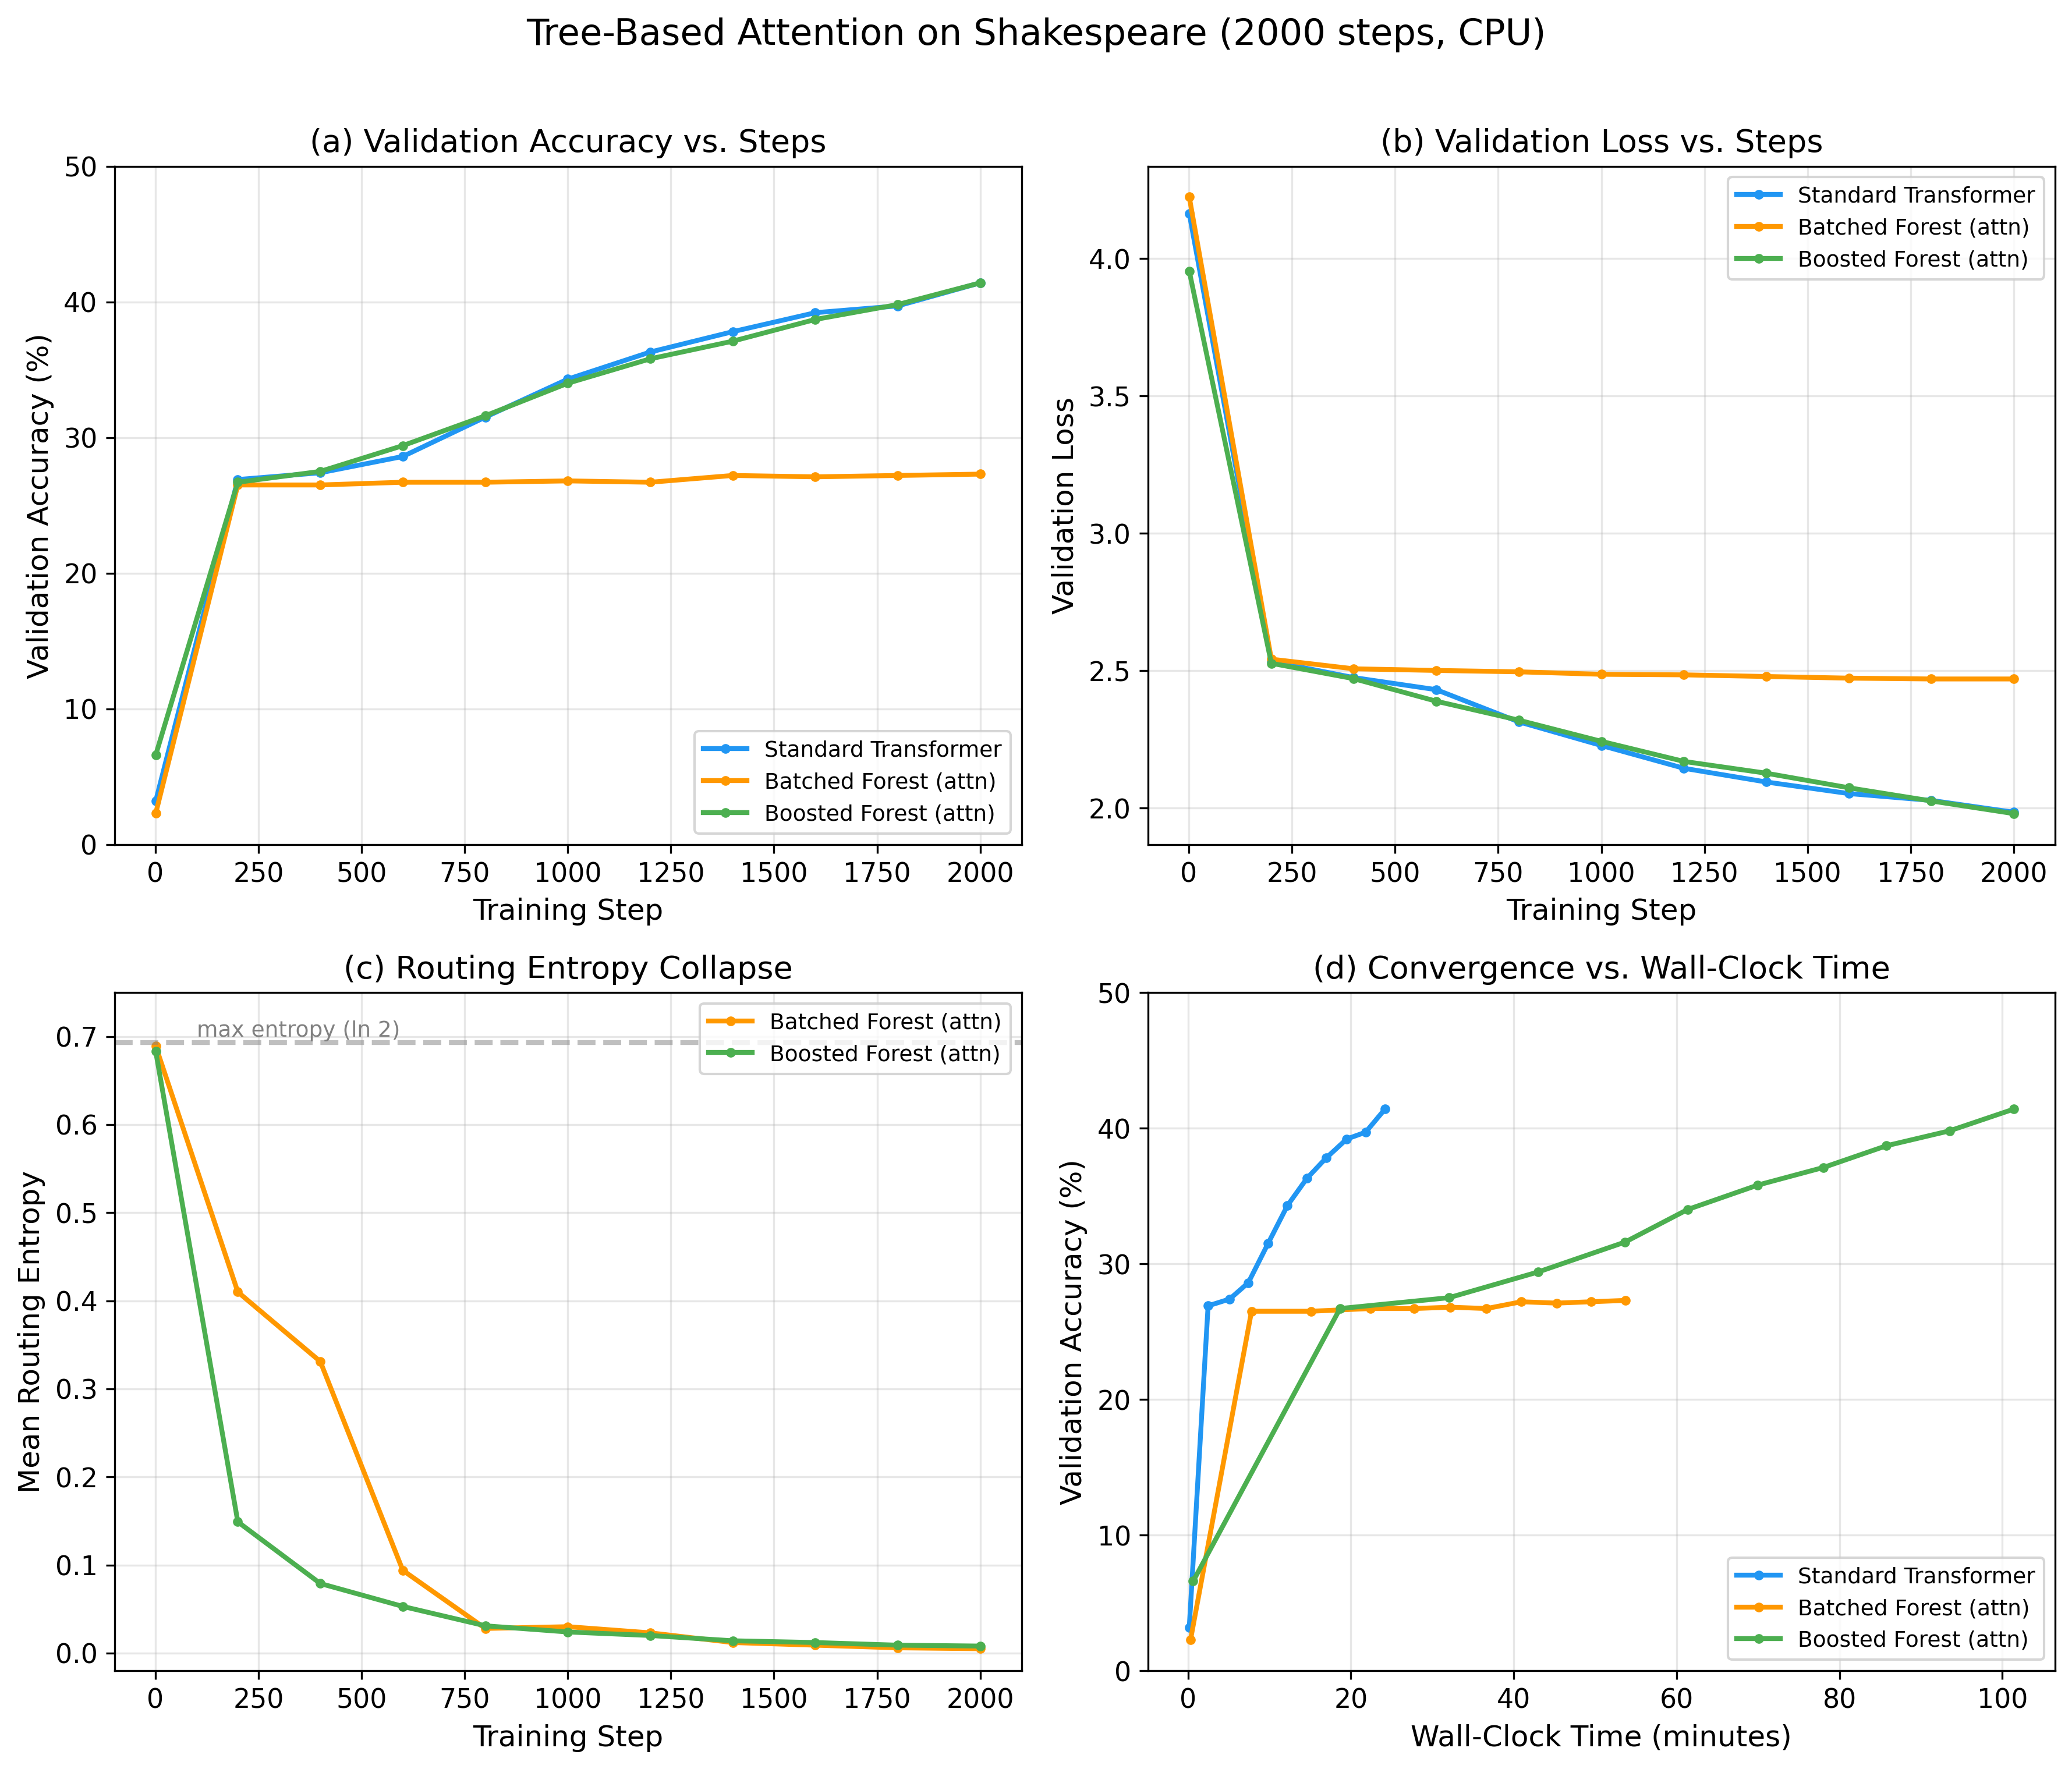
\includegraphics[width=\textwidth]{figures/main_results.png}
    \caption{Main results on Shakespeare character-level language modeling (2000 training steps, CPU). (a)~Validation accuracy vs.\ training steps. (b)~Validation loss vs.\ steps. (c)~Routing entropy collapse in tree-based models. (d)~Convergence vs.\ wall-clock time.}
    \label{fig:main}
\end{figure}

\begin{table}[H]
\centering
\caption{Shakespeare results after 2000 training steps.}
\begin{tabular}{lcccc}
\toprule
\textbf{Model} & \textbf{Val Accuracy} & \textbf{Val Loss} & \textbf{ms/step} & \textbf{Slowdown} \\
\midrule
Standard Transformer & \textbf{41.3\%} & \textbf{1.986} & 726 & $1.0\times$ \\
Batched Forest (attn) & 27.4\% & 2.471 & 1{,}611 & $2.2\times$ \\
Boosted Forest (attn) & \textbf{41.1\%} & \textbf{1.987} & 3{,}042 & $4.2\times$ \\
\bottomrule
\end{tabular}
\label{tab:results}
\end{table}

The Boosted Forest achieves validation accuracy within 0.2 percentage points of the standard transformer, demonstrating that tree-based projections can match linear projections on real language data when properly configured.

\subsection{Failure Mode: Premature Entropy Collapse}

The pure Batched Forest plateaus at 27.4\% accuracy---substantially below the standard transformer. Analysis reveals the cause: routing entropy drops from 0.69 to 0.005 over training (Figure~\ref{fig:main}c), meaning the soft trees become effectively hard decision trees within the first few hundred steps. Once routing decisions harden, the trees cannot adapt their feature partitioning, and learning stalls.

The Boosted Forest exhibits the same entropy collapse but does not suffer the same accuracy degradation. The linear base projection continues to learn throughout training, regardless of tree routing entropy. Tree stages provide incremental corrections early in training when routing is soft, and the learned shrinkage factors regulate tree influence after hardening.

\subsection{Speed Analysis}

\begin{figure}[H]
    \centering
    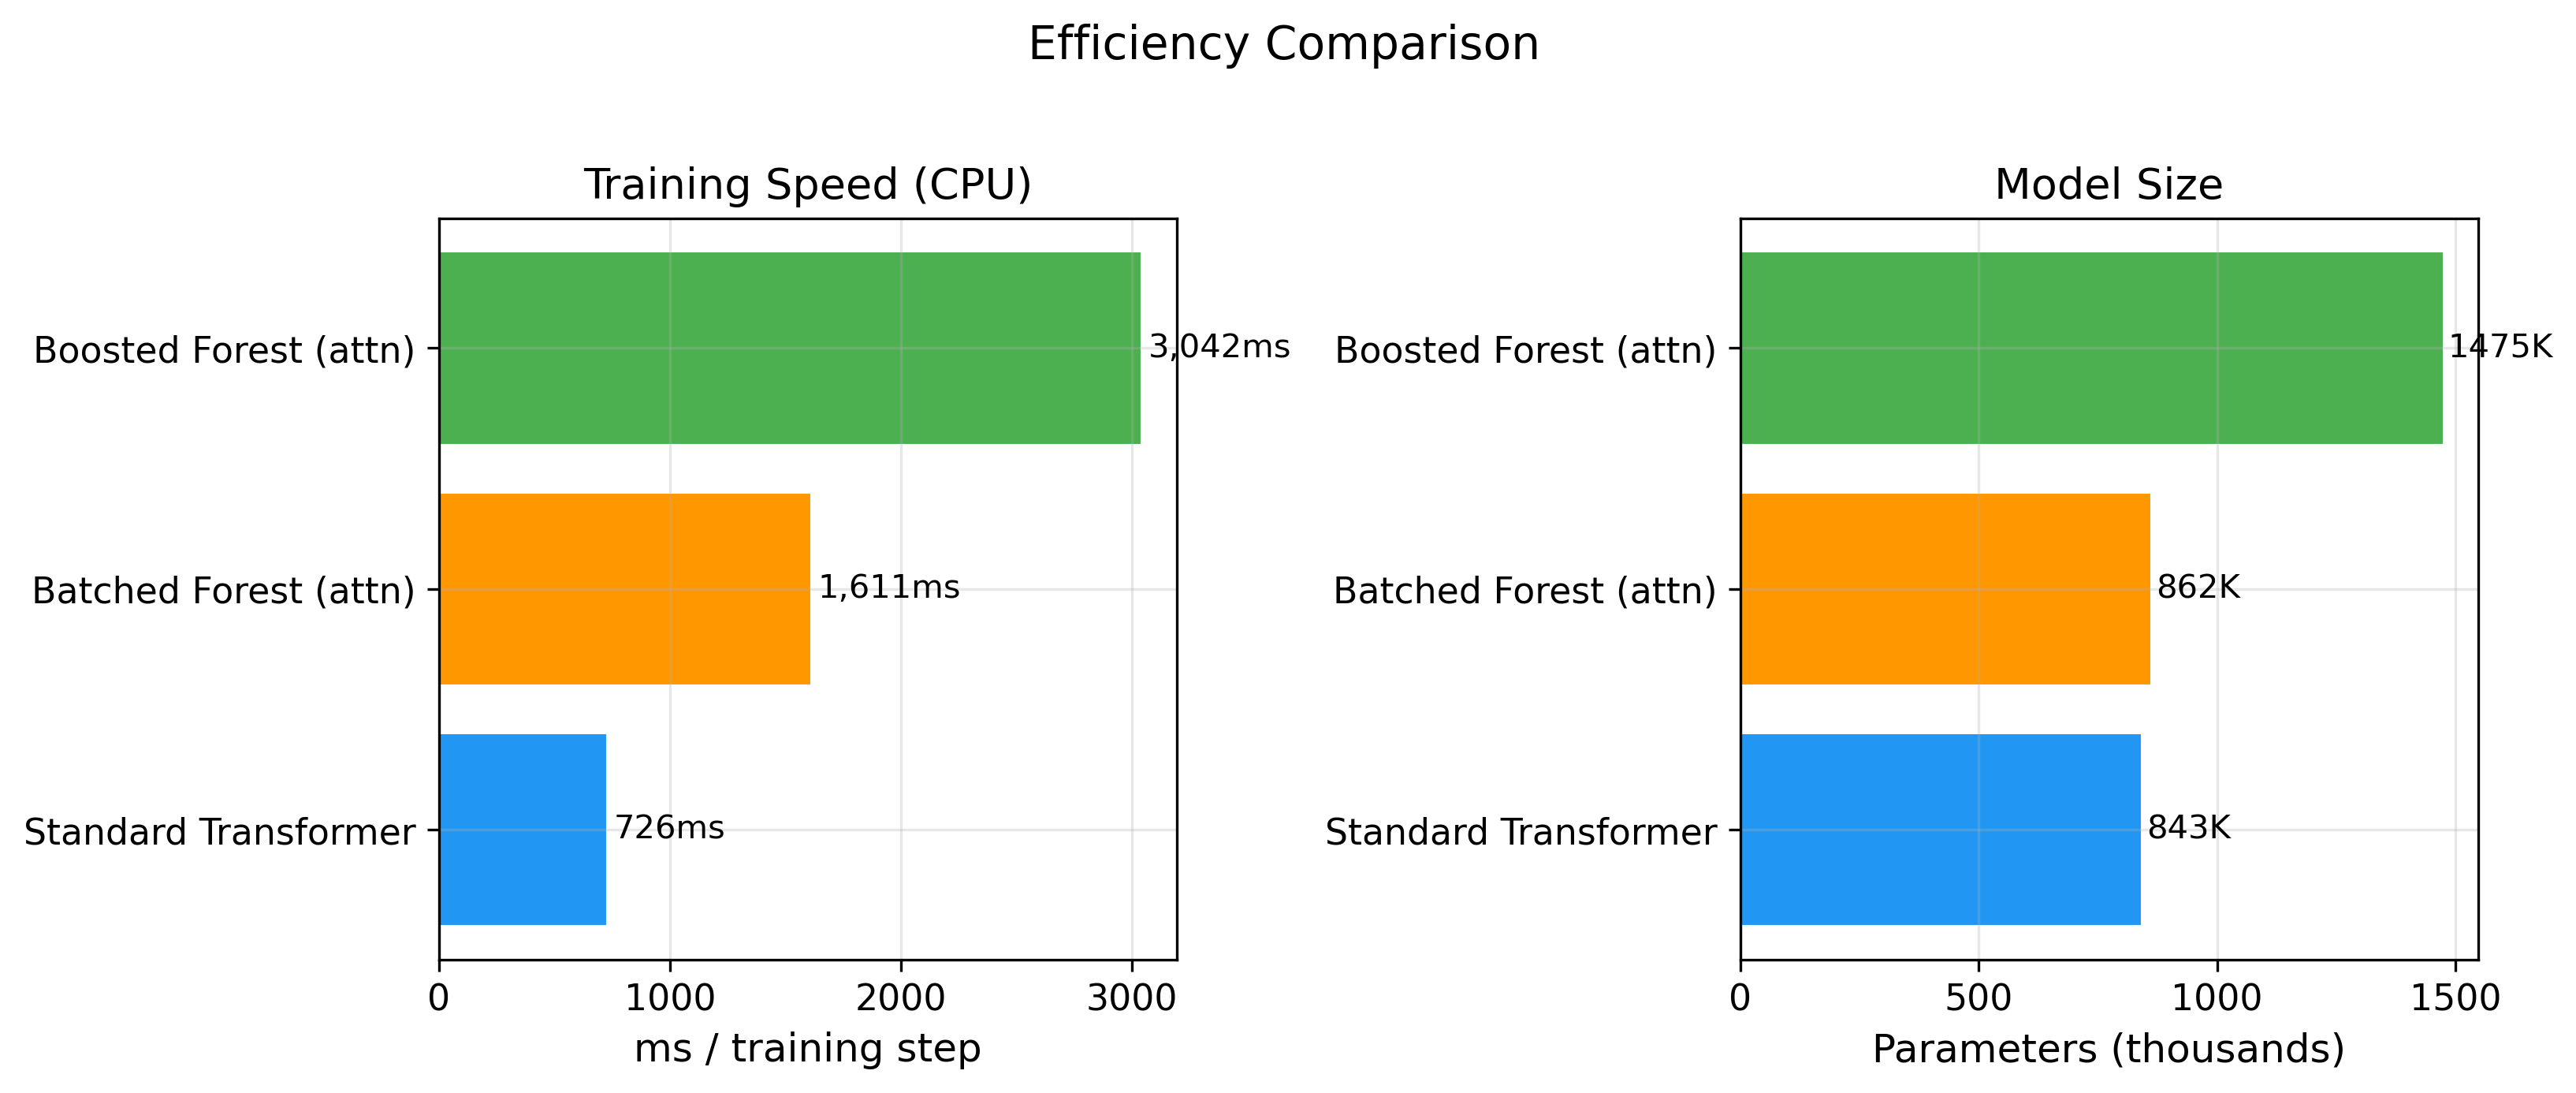
\includegraphics[width=\textwidth]{figures/speed_comparison.png}
    \caption{Training speed and model size comparison. QKV fusion reduces tree overhead from $\sim\!8\times$ to $\sim\!4\times$ vs.\ standard attention.}
    \label{fig:speed}
\end{figure}

QKV fusion reduces the attention projection from 4 separate forest forward passes to 2 (one fused QKV, one output). The remaining 4.2$\times$ gap comes from the depth loop in leaf probability computation and the three sequential boosted stages with feature pass-through.

\subsection{Synthetic Task Results}

\begin{table}[H]
\centering
\caption{Synthetic next-token prediction accuracy (vocab=256, 1000 steps).}
\begin{tabular}{lcc}
\toprule
\textbf{Task} & \textbf{Standard} & \textbf{Boosted Forest} \\
\midrule
Linear: $(prev + offset) \bmod vocab$ & 19.4\% & \textbf{20.8\%} \\
Non-linear: $\text{table}[prev \oplus prev_{prev}]$ & \textbf{2.3\%} & 2.5\% \\
\bottomrule
\end{tabular}
\end{table}

% ══════════════════════════════════════════════════════════════════════════
\section{Analysis and Discussion}

\subsection{Why Boosted Forest Works}

The success of the Boosted Forest architecture can be attributed to three design decisions:
\begin{enumerate}
    \item \textbf{Linear base provides a guaranteed gradient path.} Even if all tree routing collapses, the linear projection continues to receive clean gradients.
    \item \textbf{Residual pass-through enables correction learning.} By concatenating the current output with the original input, each tree stage can identify where the linear base's prediction is weakest.
    \item \textbf{Learned shrinkage controls tree influence.} The shrinkage parameters ($\gamma_s$, initialized at 0.1) automatically reduce tree influence if trees are not contributing useful corrections.
\end{enumerate}

\subsection{Why Pure Tree Projections Fail}

The Batched Forest's poor performance stems from a conflict between temperature annealing and optimization dynamics. As temperature drops, routing decisions sharpen and trees begin partitioning the input space based on patterns learned from limited early data. Once routing is essentially hard, the partition boundaries are frozen and recovery from suboptimal early routing is impossible. This is analogous to the ``rich get richer'' problem in mixture models.

\subsection{Implications}

Our results suggest that trees are most effective as \textit{corrections to strong base models} rather than standalone replacements. This aligns with the gradient boosting literature, where trees correct residuals of simpler models. The architectural pattern---linear base + tree corrections---may generalize beyond attention to any component where non-linear refinement of a linear operation is desired.

\subsection{Limitations}

\begin{enumerate}
    \item \textbf{Speed.} The 4.2$\times$ CPU slowdown makes pure tree-based attention impractical without GPU optimization and kernel fusion.
    \item \textbf{Scale.} Our experiments use small models (843K--1.5M parameters). Scaling behavior at larger sizes is unknown.
    \item \textbf{Temperature sensitivity.} The cosine annealing schedule is not optimized; entropy collapse suggests the minimum temperature should be higher.
    \item \textbf{Interpretability.} While trees offer the promise of interpretable routing, entropy collapse makes late-training routing essentially fixed rather than meaningfully interpretable.
\end{enumerate}

% ══════════════════════════════════════════════════════════════════════════
\section{Related Work}

\textbf{Soft Decision Trees.} \citet{irsoy2012soft} introduced soft decision trees for neural networks. \citet{frosst2017distilling} used them for distilling neural networks. \citet{hazimeh2020tree} proposed differentiable trees for tabular data.

\textbf{Tree-based Neural Networks.} Deep Neural Decision Forests \citep{kontschieder2015deep} combined random forests with neural feature learning. Adaptive Neural Trees \citep{tanno2019adaptive} learned tree structure alongside parameters.

\textbf{Mixture of Experts.} BoostedForest shares conceptual similarity with MoE \citep{shazeer2017outrageously}, where tree routing serves as a continuous form of expert selection.

\textbf{Efficient Attention.} Various alternatives to standard projections exist including low-rank \citep{wang2020linformer}, sparse \citep{child2019generating}, and kernel-based \citep{katharopoulos2020transformers} methods. Tree-based projections offer a distinct inductive bias---piecewise-constant feature partitioning.

% ══════════════════════════════════════════════════════════════════════════
\section{Future Work}

\begin{enumerate}
    \item \textbf{Shared routing:} All trees share routing decisions but have separate leaf outputs, reducing routing computation by $T\times$.
    \item \textbf{Conditional tree selection (MoTE):} Route each token to its top-$K$ most relevant trees, reducing compute from $O(T)$ to $O(K)$.
    \item \textbf{GPU optimization:} Mixed precision training and \texttt{torch.compile} could significantly close the speed gap.
    \item \textbf{Larger scale:} Evaluate on larger models and datasets to determine whether trees provide increasing benefit at scale.
    \item \textbf{Routing analysis:} Investigate what linguistic features tree routing learns to partition on.
\end{enumerate}

% ══════════════════════════════════════════════════════════════════════════
\section{Conclusion}

We demonstrate that differentiable decision trees can serve as effective projection layers in transformer attention, matching standard linear projections on character-level Shakespeare language modeling (41.1\% vs.\ 41.3\% validation accuracy). The key architectural insight is that trees work best as residual corrections to a linear base---not as standalone replacements. This Boosted Forest architecture provides a robust gradient path through the linear base while allowing trees to learn complementary non-linear patterns.

While the current implementation incurs a 4.2$\times$ speed penalty on CPU, the approach opens a new direction in transformer design: hybrid architectures that combine the efficiency of linear projections with the expressive power of learned feature partitioning.

% ══════════════════════════════════════════════════════════════════════════
\bibliographystyle{plainnat}
\begin{thebibliography}{99}

\bibitem[Child et al.(2019)]{child2019generating}
Child, R., Gray, S., Radford, A., \& Sutskever, I. (2019).
Generating long sequences with sparse transformers.
\textit{arXiv:1904.10509}.

\bibitem[Frosst \& Hinton(2017)]{frosst2017distilling}
Frosst, N. \& Hinton, G. (2017).
Distilling a neural network into a soft decision tree.
\textit{CEx Workshop, AI*IA}.

\bibitem[Hazimeh et al.(2020)]{hazimeh2020tree}
Hazimeh, H., Ponomareva, N., Mol, P., Tan, Z., \& Mazumder, R. (2020).
The tree ensemble layer: Differentiability meets conditional computation.
\textit{ICML}.

\bibitem[Irsoy et al.(2012)]{irsoy2012soft}
Irsoy, O., Y{\i}ld{\i}z, O.\,T., \& Alpaydin, E. (2012).
Soft decision trees.
\textit{ICPR}.

\bibitem[Karpathy(2015)]{karpathy2015}
Karpathy, A. (2015).
The unreasonable effectiveness of recurrent neural networks.
\textit{Blog post}.

\bibitem[Katharopoulos et al.(2020)]{katharopoulos2020transformers}
Katharopoulos, A., Vyas, A., Pappas, N., \& Fleuret, F. (2020).
Transformers are RNNs: Fast autoregressive transformers with linear attention.
\textit{ICML}.

\bibitem[Kontschieder et al.(2015)]{kontschieder2015deep}
Kontschieder, P., Fiterau, M., Criminisi, A., \& Bul\`{o}, S.\,R. (2015).
Deep neural decision forests.
\textit{ICCV}.

\bibitem[Shazeer et al.(2017)]{shazeer2017outrageously}
Shazeer, N., Mirhoseini, A., Maziarz, K., et al. (2017).
Outrageously large neural networks: The sparsely-gated mixture-of-experts layer.
\textit{ICLR}.

\bibitem[Tanno et al.(2019)]{tanno2019adaptive}
Tanno, R., Arulkumaran, K., Alexander, D.\,C., Criminisi, A., \& Nori, A. (2019).
Adaptive neural trees.
\textit{ICML}.

\bibitem[Vaswani et al.(2017)]{vaswani2017attention}
Vaswani, A., Shazeer, N., Parmar, N., et al. (2017).
Attention is all you need.
\textit{NeurIPS}.

\bibitem[Wang et al.(2020)]{wang2020linformer}
Wang, S., Li, B.\,Z., Khabsa, M., Fang, H., \& Ma, H. (2020).
Linformer: Self-attention with linear complexity.
\textit{arXiv:2006.04768}.

\end{thebibliography}

\end{document}
